\documentclass{article}\usepackage[]{graphicx}\usepackage[]{color}
%% maxwidth is the original width if it is less than linewidth
%% otherwise use linewidth (to make sure the graphics do not exceed the margin)
\makeatletter
\def\maxwidth{ %
  \ifdim\Gin@nat@width>\linewidth
    \linewidth
  \else
    \Gin@nat@width
  \fi
}
\makeatother

\definecolor{fgcolor}{rgb}{0.345, 0.345, 0.345}
\newcommand{\hlnum}[1]{\textcolor[rgb]{0.686,0.059,0.569}{#1}}%
\newcommand{\hlstr}[1]{\textcolor[rgb]{0.192,0.494,0.8}{#1}}%
\newcommand{\hlcom}[1]{\textcolor[rgb]{0.678,0.584,0.686}{\textit{#1}}}%
\newcommand{\hlopt}[1]{\textcolor[rgb]{0,0,0}{#1}}%
\newcommand{\hlstd}[1]{\textcolor[rgb]{0.345,0.345,0.345}{#1}}%
\newcommand{\hlkwa}[1]{\textcolor[rgb]{0.161,0.373,0.58}{\textbf{#1}}}%
\newcommand{\hlkwb}[1]{\textcolor[rgb]{0.69,0.353,0.396}{#1}}%
\newcommand{\hlkwc}[1]{\textcolor[rgb]{0.333,0.667,0.333}{#1}}%
\newcommand{\hlkwd}[1]{\textcolor[rgb]{0.737,0.353,0.396}{\textbf{#1}}}%

\usepackage{framed}
\makeatletter
\newenvironment{kframe}{%
 \def\at@end@of@kframe{}%
 \ifinner\ifhmode%
  \def\at@end@of@kframe{\end{minipage}}%
  \begin{minipage}{\columnwidth}%
 \fi\fi%
 \def\FrameCommand##1{\hskip\@totalleftmargin \hskip-\fboxsep
 \colorbox{shadecolor}{##1}\hskip-\fboxsep
     % There is no \\@totalrightmargin, so:
     \hskip-\linewidth \hskip-\@totalleftmargin \hskip\columnwidth}%
 \MakeFramed {\advance\hsize-\width
   \@totalleftmargin\z@ \linewidth\hsize
   \@setminipage}}%
 {\par\unskip\endMakeFramed%
 \at@end@of@kframe}
\makeatother

\definecolor{shadecolor}{rgb}{.97, .97, .97}
\definecolor{messagecolor}{rgb}{0, 0, 0}
\definecolor{warningcolor}{rgb}{1, 0, 1}
\definecolor{errorcolor}{rgb}{1, 0, 0}
\newenvironment{knitrout}{}{} % an empty environment to be redefined in TeX

\usepackage{alltt}
\IfFileExists{upquote.sty}{\usepackage{upquote}}{}
\begin{document}

\title {Change in Historical Average Federal Tax Rates for All Households} 
\author { Paul Wagner  
\\ School of Information Technology 
\\ Illinois State University
\\
\texttt{pgwagne@ilstu.edu}}
\date{\today} 
\maketitle

The average federal tax rate is calculated by federal tax liabilities divided by pre-tax income of a household. This tax rate has been divided into five categories by the CBO to illustrate tax burden on various income levels. These statistics illustrate the change from 1970 of three of the five tax brackets. The Lowest Quintile, Top Quintile and all Quintiles combined. 

\section{Obtaining the data}



\begin{knitrout}
\definecolor{shadecolor}{rgb}{0.969, 0.969, 0.969}\color{fgcolor}\begin{kframe}
\begin{alltt}
\hlstd{x} \hlkwb{<-} \hlkwd{getURL}\hlstd{(}\hlstr{"https://www.quandl.com/api/v1/datasets/TPC/HIST_FED_TAX_IND_ITR.csv"}\hlstd{)}
\hlstd{taxdata} \hlkwb{<-} \hlkwd{read.csv}\hlstd{(}\hlkwc{text} \hlstd{= x)}
\end{alltt}
\end{kframe}
\end{knitrout}

\section{Data}

\subsection{Data Description}

The data includes three columns of numbers. These values are based off of a percentage of change or difference starting from 1979 the Lowest Quintile, 0, all quintiles, 4 and the top 1\%, 7.4. The data does not represent the actual tax rate paid by each quintile. Representation of this data may be confusing as the graph is only showing a change of tax rates and not an actual tax rate. To illustrate the data better, in 2010: the lowest quintile paid 1.5\% federal tax rate while the top 1\% paid a federal tax rate of 29.4\%.

The allowable value of the first column is a date - a 4 digit year, followed by a 2 digit month and a 2 digit day. The allowable values for columns 2, 3 and 4 are positive or negative numbers with a single digit after the decimal point.

\subsection{Data Exploration}


\begin{knitrout}
\definecolor{shadecolor}{rgb}{0.969, 0.969, 0.969}\color{fgcolor}\begin{kframe}
\begin{alltt}
\hlkwd{class}\hlstd{(taxdata.new)}
\end{alltt}
\begin{verbatim}
## [1] "data.frame"
\end{verbatim}
\begin{alltt}
\hlkwd{str}\hlstd{(taxdata.new,} \hlkwc{width} \hlstd{=} \hlnum{60}\hlstd{,} \hlkwc{strict.width} \hlstd{=} \hlstr{"wrap"}\hlstd{)}
\end{alltt}
\begin{verbatim}
## 'data.frame':	32 obs. of  4 variables:
## $ Year : Factor w/ 32 levels "1979-12-31","1980-12-31",..:
##    32 31 30 29 28 27 26 25 24 23 ...
## $ Lowest.Quintile: num -9.2 -9.3 -9.1 -5.8 -5.7 -5.7 -5.4
##    -5.4 -5.2 -4.9 ...
## $ All.Quintiles : num -2.3 -2.6 -2.5 -0.1 -0.4 -0.5 -0.5
##    -0.7 0.1 0.5 ...
## $ Top.1..  : num 1.6 1.3 1.2 3.1 2.9 2.8 2.8 2.7 3.5 3.8
##    ...
\end{verbatim}
\begin{alltt}
\hlkwd{summary}\hlstd{(taxdata.new)}
\end{alltt}
\begin{verbatim}
##          Year    Lowest.Quintile  All.Quintiles   
##  1979-12-31: 1   Min.   :-9.300   Min.   :-2.600  
##  1980-12-31: 1   1st Qu.:-5.250   1st Qu.: 0.050  
##  1981-12-31: 1   Median :-3.400   Median : 2.000  
##  1982-12-31: 1   Mean   :-3.075   Mean   : 1.747  
##  1983-12-31: 1   3rd Qu.:-0.300   3rd Qu.: 3.400  
##  1984-12-31: 1   Max.   : 0.700   Max.   : 4.700  
##  (Other)   :26                                    
##     Top.1..    
##  Min.   :1.20  
##  1st Qu.:3.40  
##  Median :5.25  
##  Mean   :4.95  
##  3rd Qu.:6.05  
##  Max.   :8.20  
## 
\end{verbatim}
\end{kframe}
\end{knitrout}

\section{Results}

\begin{table}

\begin{knitrout}
\definecolor{shadecolor}{rgb}{0.969, 0.969, 0.969}\color{fgcolor}\begin{kframe}
\begin{verbatim}
taxdata.new
##          Year Lowest.Quintile All.Quintiles Top.1..
## 1  2010-12-31            -9.2          -2.3     1.6
## 2  2009-12-31            -9.3          -2.6     1.3
## 3  2008-12-31            -9.1          -2.5     1.2
## 4  2007-12-31            -5.8          -0.1     3.1
## 5  2006-12-31            -5.7          -0.4     2.9
## 6  2005-12-31            -5.7          -0.5     2.8
## 7  2004-12-31            -5.4          -0.5     2.8
## 8  2003-12-31            -5.4          -0.7     2.7
## 9  2002-12-31            -5.2           0.1     3.5
## 10 2001-12-31            -4.9           0.5     3.8
## 11 2000-12-31            -4.0           1.5     4.9
## 12 1999-12-31            -4.5           1.7     4.9
## 13 1998-12-31            -4.6           1.6     4.9
## 14 1997-12-31            -4.2           2.0     5.4
## 15 1996-12-31            -4.2           1.9     5.2
## 16 1995-12-31            -3.6           2.0     5.2
## 17 1994-12-31            -3.2           1.9     5.2
## 18 1993-12-31            -1.7           2.2     5.3
## 19 1992-12-31            -1.6           2.4     5.4
## 20 1991-12-31            -1.2           2.8     5.7
## 21 1990-12-31            -0.7           3.3     5.9
## 22 1989-12-31            -1.3           2.9     5.9
## 23 1988-12-31            -0.9           3.0     5.9
## 24 1987-12-31            -0.4           3.1     5.8
## 25 1986-12-31             0.5           3.9     6.5
## 26 1985-12-31             0.6           3.9     6.6
## 27 1984-12-31             0.7           3.9     6.5
## 28 1983-12-31             0.4           3.7     6.6
## 29 1982-12-31             0.5           4.1     7.4
## 30 1981-12-31             0.5           4.7     8.2
## 31 1980-12-31             0.2           4.4     7.9
## 32 1979-12-31             0.0           4.0     7.4
\end{verbatim}
\end{kframe}
\end{knitrout}
\caption{Change in Federal Tax Rates}
\label{table:table1}
\end{table}

Income quintiles are calculated by ranking households by income and adjusting for the number of members of the household by dividing by the square root of the household’s size. All quintiles contain the same number of people. Households who have negative income in a year are excluded from the lowest quintile but included in totals.

\section{Plotting the data}

\begin{table}
\begin{knitrout}
\definecolor{shadecolor}{rgb}{0.969, 0.969, 0.969}\color{fgcolor}
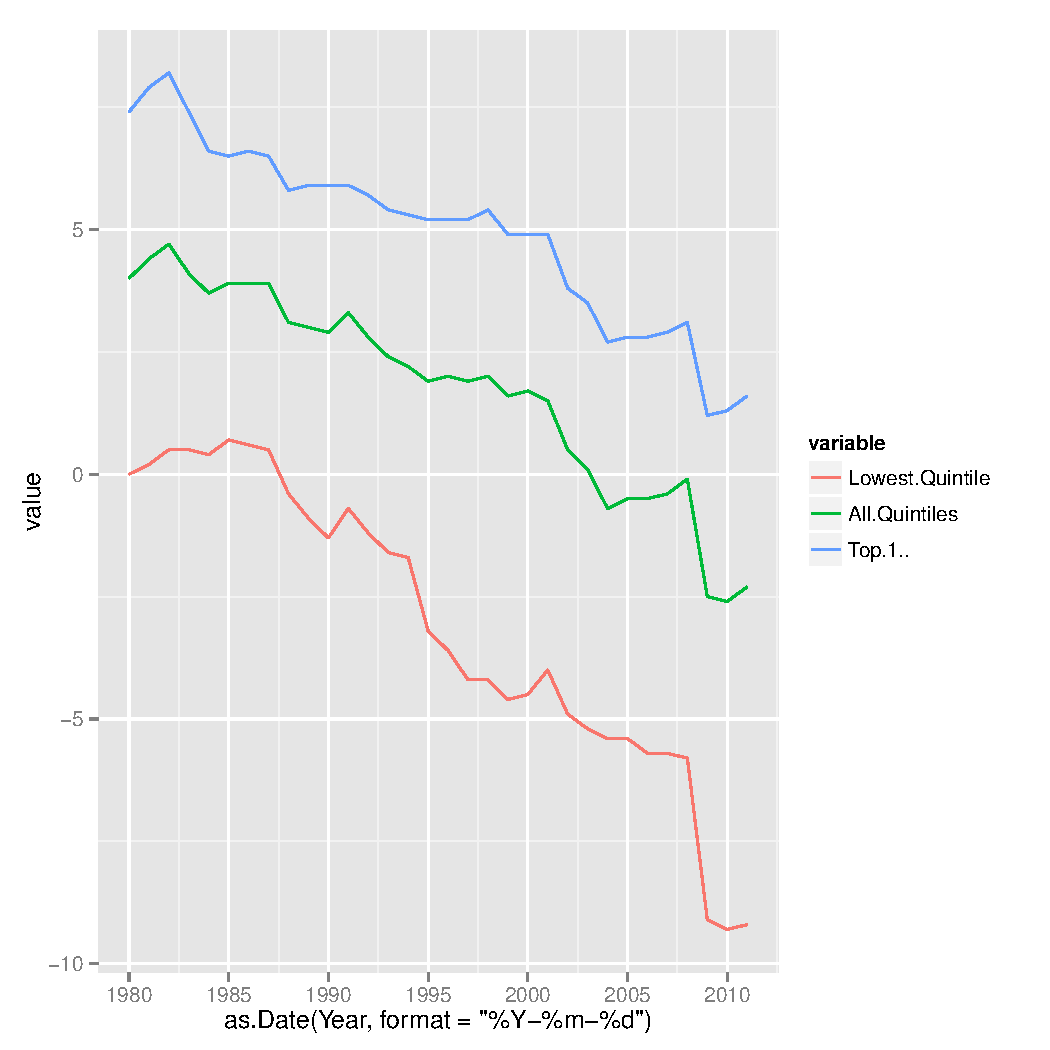
\includegraphics[width=\maxwidth]{figure/unnamed-chunk-6-1} 

\end{knitrout}
\caption{Change in Lowest Quintile, All Quintiles, Top 1\% Rates}
\label{table:graph1}
\end{table}

\subsection{Data Conclusions}

Taxes were raised on the wealthy in 1993 by adding two new tax brackets on the top which manifests itself as a less dramatic drop to the top 1\% rate as compared to the overall and lowest brackets over the same time period. Taxes were cut in 2001 through 2003, which lowered overall taxes which is shown in the data. The crash and beginning of the recession is illustrated in table \ref{table:graph1} on page \pageref{table:graph1} by the dramatic overall drop from 2008 to 2010.

Since the data in table \ref{table:table1} on page \pageref{table:table1} shows taxes earned, which directly correlates to income earned, these numbers give a good indication of overall economic health as much as they do about large changes to tax policy in the United States. Adjusted for inflation, income for the middle quintile down have remained generally flat since 1970 whereas higher income earners in the top quintile and top 1\% have seen their incomes rise 30-40\%. Lower income earners were hurt much more by the recession as compared to the top 1\% of earners.


\end{document}
